\documentclass[12pt]{article}

\usepackage{amsmath}
\usepackage{amssymb}
\usepackage{graphicx}
\usepackage{tikz}
\usetikzlibrary{shapes.geometric, arrows}
\usepackage{forest}

\tikzstyle{fit} = [rectangle, inner sep = 0.2cm, rounded corners, minimum height = 0.6cm, text centered, draw = black, fill = cyan!20]
\tikzstyle{tree} = [rectangle, inner sep = 0.2cm, rounded corners, minimum height = 0.6cm, text centered, draw = black, fill = green!20]
%\tikzstyle{ellip} = [rectangle, inner sep = 0.2cm, minimum height = 0.6cm, text centered]

\setlength{\parskip}{6pt}

\begin{document}
\[
	\text{RSS} = \sum\limits_{i = 1}^n \Big( y_i - (\beta_0 + \beta_1 x_1 + \beta_2 x_2 + \cdots + \beta_p x_p)\Big)^2
\]

\[
\text{minimize}\quad \underbrace{\sum\limits_{i = 1}^n \Big( y_i - (\beta_0 + \beta_1 x_1 + \beta_2 x_2 + \cdots + \beta_p x_p)\Big)^2}_{\text{residual sum of squares}} + \underbrace{\sum\limits_{j = 1}^p \vert \beta_j \vert}_{\text{penalty}}
\]

\[
	\text{minimize}\quad \underbrace{\sum\limits_{i = 1}^n \Big( y_i - (\beta_0 + \beta_1 x_1 + \beta_2 x_2 + \cdots + \beta_p x_p)\Big)}_{\text{residual sum of squares}}\quad \text{where}\quad  \underbrace{\sum\limits_{j = 1}^p \vert \beta_j\vert \leq t}_{\text{penalty}}
\]



\[
\text{minimize}\quad \underbrace{\sum\limits_{i = 1}^n \Big( y_i - (\beta_0 + \beta_1 x_1 + \beta_2 x_2 + \cdots + \beta_p x_p)\Big)^2}_{\text{residual sum of squares}} + \underbrace{\sum\limits_{j = 1}^p P(\beta_j)}_{\text{penalty}}
\]

\[
	\underbrace{E(y_0 - \hat{y}_0)}_{\text{expected residual}}=\underbrace{\text{Var}(\hat{y}_0)}_{\text{variance of model}} + \underbrace{(\text{Bias}(\hat{y}_0))^2}_{\text{squared bias of model}} + \underbrace{\text{Var}(\epsilon)}_{\text{variance of error}}
\]

\[
	\hat{\beta} = (\mathbf{X}^\top\mathbf{X})^{-1}\mathbf{X}^\top \mathbf{y}
\]

\[
	Y = \beta_0 + \beta_1 X_1 + \beta_2 X_2 + \cdots + \beta_p X_p + \epsilon
\]

\newpage

Let $n$ be an integer. Prove that $4\nmid n^2 - 3$.

We will consider three cases. First, assume that $n$ is even. Then $n = 2k$ for some integer $k$. Hence,
\begin{align}
	n^2 - 3 &= (2k)^2 - 3 \\
	&= 4k^2 - 3
\end{align}
which is not a multiple of 4.

Now, assume that $n$ is odd. Then $n = 2k + 1$ for some integer $k$. Then
\begin{align}
	n^2 - 3 &= (4k + 1)^2 - 3 \\
	&= (16k^2 + 8k + 1) - 3\\
	&= 16k^2 + 8k - 2\\
	&= 4(4k^2 + 2k) - 2
\end{align}
which is also not a multiple of 4. Thus, for all integers $n$, $n^2 - 3$ is not a multiple of four. Therefore, $4\nmid n^2 - 3$ for all integers $n$.

\newpage
\begin{figure}
\footnotesize
\centering
\begin{forest}
	[Test observation,inner sep = 0.2cm, rounded corners, minimum height = 0.6cm, draw = black, fill = cyan!20
		%Tree 1
		[,circle,draw,fill=cyan,edge={->},label=Tree 1
			[,circle,draw,fill=cyan
				[,circle,draw
					[,circle,draw]
					[,circle,draw]
				]
				[,circle,draw,fill=cyan
					[,circle,draw]
					[,circle,draw,fill=cyan
						[Prediction 1,edge={->},inner sep = 0.2cm, rounded corners, minimum height = 0.6cm, draw = black, fill = green!20] {
							\draw[->] () to (agg);
						}
					]
				]
			]
			[,circle,draw
				[,circle,draw
					[,circle,draw]
					[,circle,draw]
				]
				[,circle,draw
					[,circle,draw]
					[,circle,draw]
				]
			]
		]
		% Tree 2
		[,circle,draw,fill=cyan,edge={->},label={[xshift=-2em,font=\small]Tree 2}
			[,circle,draw
				[,circle,draw
					[,circle,draw]
					[,circle,draw]
				]
				[,circle,draw
					[,circle,draw]
					[,circle,draw]
				]
			]
			[,circle,draw,fill=cyan
				[,circle,draw,fill=cyan
					[,circle,draw]
					[,circle,draw,fill=cyan
						[Prediction 2,edge={->},inner sep = 0.2cm, rounded corners, minimum height = 0.6cm, draw = black, fill = green!20
							[Aggregate result,edge={->},inner sep = 0.2cm, rounded corners, minimum height = 0.6cm, draw = black, fill = cyan!20,name=agg]
						]
					]
				]
				[,circle,draw
					[,circle,draw]
					[,circle,draw]
				]
			]
		]
		[..., l*=2,edge={->},inner sep = 0.2cm, rounded corners, minimum height = 0.6cm, draw = black, fill = cyan!20
			[...,l*=3,edge={->},inner sep = 0.2cm, rounded corners, minimum height = 0.6cm, draw = black, fill = green!20] {
				\draw[->] () to (agg);
			}
		]
		% Tree 3
		[,circle,draw,fill=cyan,edge={->},label=Tree $k$
			[,circle,draw
				[,circle,draw
					[,circle,draw]
					[,circle,draw]
				]
				[,circle,draw
					[,circle,draw]
					[,circle,draw]
				]
			]
			[,circle,draw,fill=cyan
				[,circle,draw
					[,circle,draw]
					[,circle,draw]
				]
				[,circle,draw,fill=cyan
					[,circle,draw]
					[,circle,draw,fill=cyan
						[Prediction $k$,edge={->},inner sep = 0.2cm, rounded corners, minimum height = 0.6cm, draw = black, fill = green!20] {
							\draw[->] () to (agg);
						}
					]
				]
			]
		]
	]
\end{forest}
\caption{Random forest}
\end{figure}

\vspace{30pt}

\begin{figure}
\footnotesize
\centering
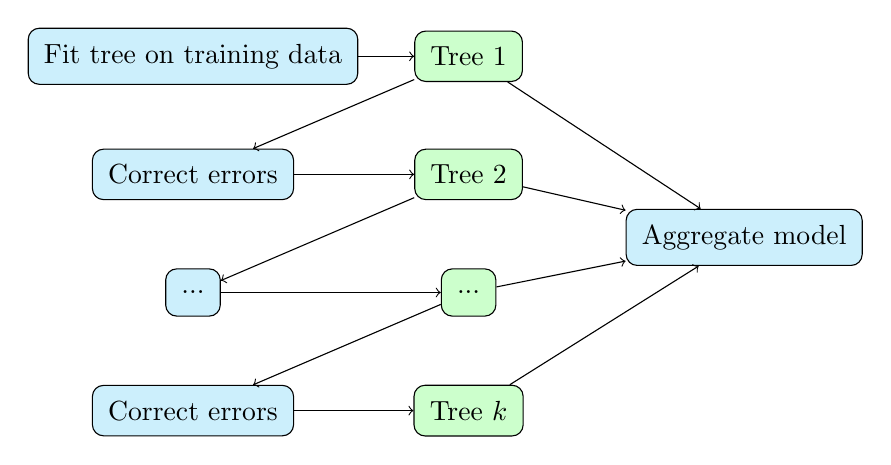
\begin{tikzpicture}
	\node (fit1)[fit]{Fit tree on training data};
	\node (tree1)[tree, right of = fit1, xshift = 2.5cm]{Tree 1};
	\node (fit2)[fit, below of = fit1, yshift = -0.5cm]{Correct errors};
	\node (tree2)[tree, right of = fit2, xshift = 2.5cm]{Tree 2};
	\node (fit3)[fit, below of = fit2, yshift = -0.5cm]{...};
	\node (tree3)[tree, right of = fit3, xshift = 2.5cm]{...};
	\node (fit4)[fit, below of = fit3, yshift = -0.5cm]{Correct errors};
	\node (tree4)[tree, right of = fit4, xshift = 2.5cm]{Tree $k$};
	\node (end)[fit, right of = tree2, xshift = 2.5cm, yshift = -0.8cm]{Aggregate model};
	
	\draw [->] (fit1) -- (tree1);
	\draw [->] (tree1) -- (fit2);
	\draw [->] (fit2) -- (tree2);
	\draw [->] (tree2) -- (fit3);
	\draw [->] (fit3) -- (tree3);
	\draw [->] (tree3) -- (fit4);
	\draw [->] (fit4) -- (tree4);
	
	\draw [->] (tree1) -- (end);
	\draw [->] (tree2) -- (end);
	\draw [->] (tree3) -- (end);
	\draw [->] (tree4) -- (end);
\end{tikzpicture}
\caption{Gradient boosting}
\end{figure}
\end{document}